\chapter{ROS и система управления}\label{ch:5}

\textit{ROS} имеет пакет MoveIT, который имеет в себе все необходимое для управления манипуляторами. В частности он включает в себя большое количество различных планировщиков путей, а также интерполятор траекторий. Кроме того, он умеет поддерживать карту окружающей среды, как полученную благодаря обработке данных с датчиков, так и фиксированную. Этот пакет и будет использован для управления \textit{UR10}.

\section{Выбор алгоритмов} \label{sect:5_1}
\begin{itemize}
	\item Планирование путей будет осуществляться с помощью RRT, поскольку это один из самых эффективных способов поиска пути.
	\item Планирование траекторий будет осуществляться с помощью интерполяции сплайнами 3-й степени.
	\item Управление реализуется я в Joint Space, а значит требуется решать задачу обратной кинематики. Используется алгоритм Damped Least-Squares, поскольку обеспечивает численную стабильность решения в области сингулярных конфигураций.
\end{itemize}
Полная схема системы управления представлена на рис. \ref{fig:5_1_1}.
\begin{figure}[h!]
	\centering
	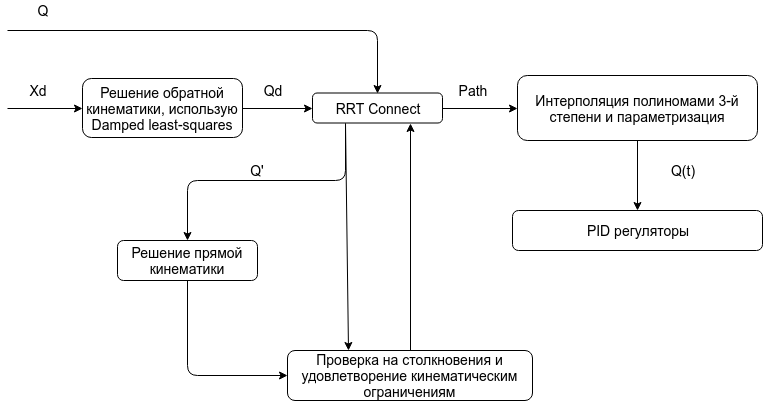
\includegraphics[scale=0.5]{ROSControl/ROS_CONTROL}
	\caption{Система управления роботом UR10}
	\label{fig:5_1_1}
\end{figure}
Система была промоделирована и протестирована в среде моделирования \textit{Gazebo}.